\documentclass[a4paper,11pt]{article}
\usepackage[utf8]{inputenc}
\usepackage{algorithmic}
\usepackage{algorithm}
\usepackage{pst-plot}
\usepackage{graphicx}
\usepackage{endnotes}
\usepackage{graphics}
\usepackage{floatflt}
\usepackage{wrapfig}
\usepackage{amsfonts}
\usepackage{amsmath}
\usepackage{amssymb}
\usepackage{verbatim}
\usepackage{hyperref}
\usepackage{multirow}
\usepackage{pdflscape}
 \usepackage{enumitem}

\usepackage{hyperref}
\hypersetup{pdfborder={0 0 0 0}}

\pdfpagewidth 210mm
\pdfpageheight 297mm 
\setlength\topmargin{0mm}
\setlength\headheight{0mm}
\setlength\headsep{0mm}
\setlength\textheight{250mm}	
\setlength\textwidth{159.2mm}
\setlength\oddsidemargin{0mm}
\setlength\evensidemargin{0mm}
\setlength\parindent{7mm}
\setlength\parskip{0mm}

\newenvironment{exercise}[3]{\paragraph{Exercise #1: #2 (#3pt)}\ \\}{
\medskip}
\newcommand{\question}[2]{\setlength\parindent{0mm}\ \\$\mathbf{Q_{#1}:}$ #2\ \\}

\author{\large{Ilya Kuzovkin, Jaan Aru}}
\title{\huge{Introduction to Computational Neuroscience}\\\LARGE{Practice IX: Memory and Perception}}

\begin{document}
\maketitle


%
% Intro
%
\ \\

\ \\
\textbf{Request:} Please record the time you will spend of this homework and add it to the report. This is just for me to balance the amount and the difficulty level of the exercises.

%
% Lecture-based questions
%
\begin{exercise}{1}{Questionnaire}{0.5}
Please provide full and detailed answers.\\
\question{1}{Explain the difference and the relationship between episodic and semantic memory.}
\question{2}{How does the Morris water maze work?}
\question{3}{Explain one candidate mechanism for working memory.}
\question{4}{Which brain area is crucial for declarative long-term memory?}
\end{exercise}


%
% Statistical significance
%
\begin{exercise}{2}{Statistical significance}{2}
The data for this exercise comes from human intracranial recordings. The electrode sits on the part of the cortex that is sensitive to human body parts. The subjects are shown pictures of persons. These pictures are made less visible with different amounts of noise on them: \texttt{deg1.mat} has more noise than \texttt{deg2.mat} (see Figure \ref{fig:noisypic}).
\begin{figure}[H]
	\centering
	
\includegraphics[width=0.8\textwidth]{noisypic.png} 
	\caption{More noise on the left (\texttt{deg1}) and less noise on the right (\texttt{deg2})}
	\label{fig:noisypic}
	\vspace{-18pt}
\end{figure}
\ \\
Thus the hypothesis is that when subjects can perceive the persons better (i.e. there is less noise) the local response in this part of the cortex should be stronger. This local response is often measured as the increased signal power in the high gamma (50-150 Hz) frequency band, so it should be that the high gamma response is stronger in trials in \texttt{deg2.mat} than trials with \texttt{deg1.mat}. Is this really so?

\ \\
Let us just have a look. The first part of the \texttt{exericse2.m} will produce Figure \ref{fig:avgheatmap},
\begin{figure}[H]
	\centering
	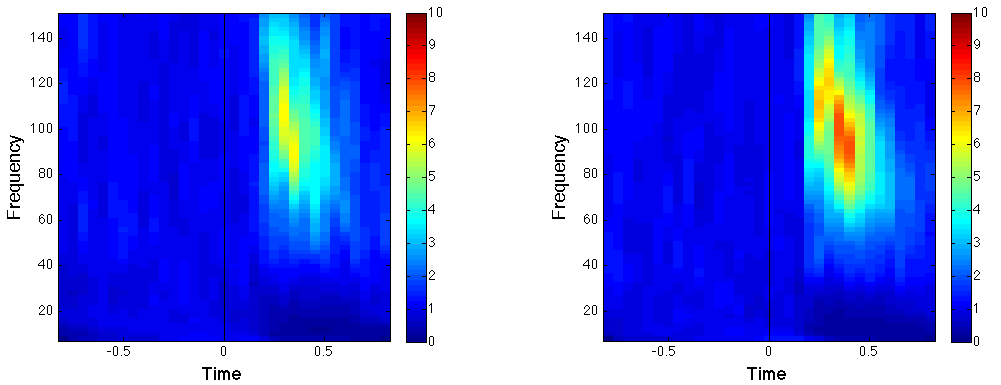
\includegraphics[width=1.0\textwidth]{avgheatmap.png}
	\caption{The activity averaged over trials. The response to the pictures with more noise (\texttt{deg1}) on left and the response to the pictures with less noise (\texttt{deg2}) on the right. The black vertical bar at the time $t=0$ indicates the moment when the stimulus was shown.}
	\label{fig:avgheatmap}
   	\vspace{-18pt}
\end{figure}
\end{exercise}
\ \\
This figure clearly shows that indeed it seems that \texttt{deg2} has higher activity in the timeframe from 200 - 600 ms after the stimulus (time moment 0) in the high gamma (50-150 Hz) frequency band.

\ \\
The big question here is whether the effect we see with our eyes indeed shows a significant result or can be attributed to random luck? How do we know where is the line between ``Yes, the activity is different" and ``No, it is just a random effect"? This is where statistical tests come into play.

\ \\
\textbf{Gentle introduction into the idea of t-test}\\
The most frequently used way to check whether your results are really different is the Student's \emph{t-test}\footnote{\url{http://en.wikipedia.org/wiki/Student's_t-test}}. There is a zoo\footnote{\url{http://en.wikipedia.org/wiki/List_of_tests\#Statistical_tests}} of them out there, but t-test is most popular due to simple equations and clear interpretation. Say you have bunch of measurements from two different conditions (for example: before and after the stimulus, one or the other stimulus, etc):
$$\text{Measurements taken during condition A: } \{a_1, a_2, \ldots, a_n\}$$
$$\text{Measurements taken during condition B: } \{b_1, b_2, \ldots, b_n\}$$
We assume that those measurements come form two normal distributions: $\mathcal{N}(\mu_A, \sigma_A)$ and $\mathcal{N}(\mu_B, \sigma_B)$ as Figure \ref{fig:twonormals} depicts.
\begin{figure}[H]
   \centering
   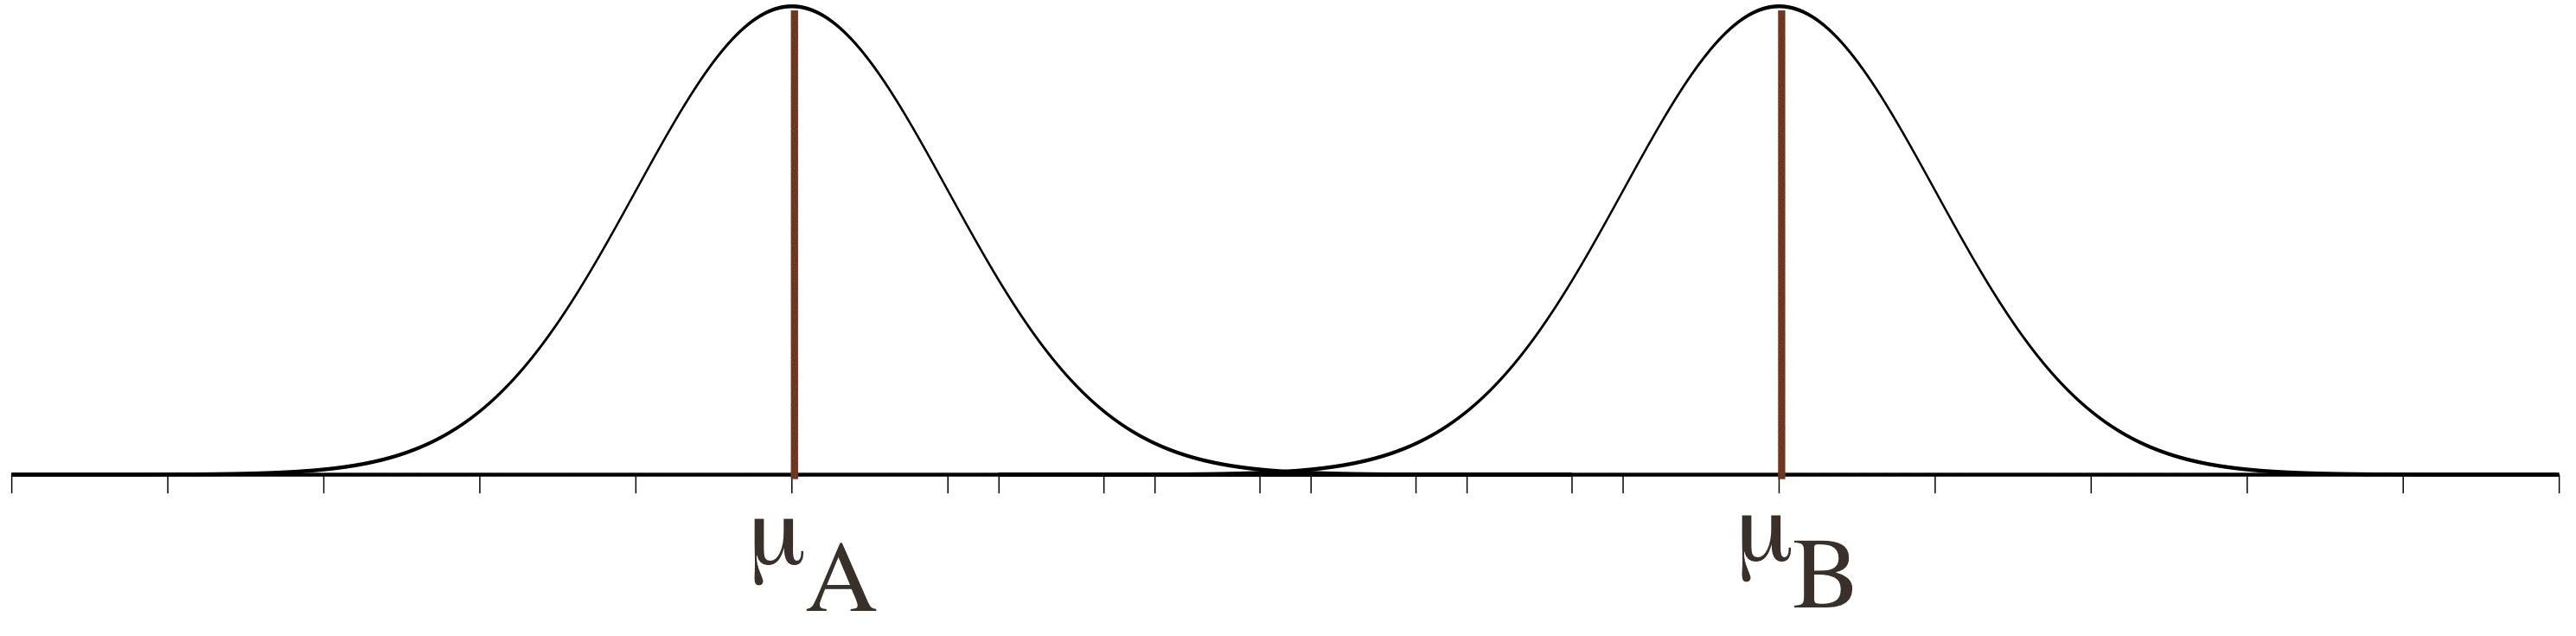
\includegraphics[width=0.8\textwidth]{twonormals.png} 
   \caption{Example of two normal distributions with means $\mu_A$ ja $\mu_B$}
   \label{fig:twonormals}
\end{figure}
\ \\
We would like to know if there is a significant difference between the means ($\mu$) of these two distributions. Statisticians say that we formulate two hypothesis:
\begin{itemize}
	\item $H_0$ is the \emph{null-hupothesis}, which correponds to the ``non-interesting" case: distributions are same.
	\item $H_1$ is the \emph{alternative hupothesis}, which correponds to the ``interesting" case: distributions are different.
\end{itemize}
\ \\
Next we compute so-called \emph{t-statistic} (note that this is the equation for the \emph{independent two-sample t-test}, which means that we have samples from two populations and that we assume that two samples are \emph{independent and identically distributed (iid)}) as follows:
$$t = \frac{\overline{a} - \overline{b}}{\sqrt{\frac{1}{2}(s^2_A + s^2_B)}\sqrt{\frac{2}{n}}}$$
where
$$\overline{a} = \texttt{mean}(\{a_1, a_2, \ldots, a_n\})$$
$$\overline{b} = \texttt{mean}(\{b_1, b_2, \ldots, b_n\})$$
$s$ is a standard deviation:
$$s_A = \texttt{sd}(\{a_1, a_2, \ldots, a_n\})$$
$$s_B = \texttt{sd}(\{b_1, b_2, \ldots, b_n\})$$
and $n$ is the total number of samples.

\ \\
Once $t$ value is determined, we can use the table of values\footnote{\url{http://en.wikipedia.org/wiki/Student's_t-distribution\#Table_of_selected_values}} of Student's t-distribution to find \emph{p-value}. P-value is the probability that distributions are same. If p-value is below some threshold of statistical significance (for example: 0.1, 0.05, 0.01), then the null hypothesis ($H_0$) is rejected in favor of the alternative hypothesis ($H_1$), which means that the ``interesting" case happened: distributions are different, since probability that they are same (p-value) is low.

\ \\
Luckily for you Matlab has a function \texttt{ttest2}, which does all that for you:
\begin{verbatim}
[H, p] = ttest([a1, a2, ..., an], [b1, b2, ..., bn])
\end{verbatim}
will say whether the alternative hypothesis is accepted (\texttt{H = 1}) and output the p-value (\texttt{p}).


\ \\
\textbf{Finally here is what you need to do in this exericse:}\\
\begin{enumerate}
	\item Feel the reason why we need to do significance testing.
	\item We have 79 trials for condition A (noisy picture) and 77 trials from condition B (less noisy picture) and we want to know if the red blob on the right part of Figure \ref{fig:avgheatmap} is significantly different from the yellow blob on the left part of this figure.
	\begin{enumerate}
		\item Each trial is represented by a matrix $72 \times 33$ where rows are frequencies and columns are the time moments (Figure \ref{fig:avgheatmap} is a visualization of such matrix).
		\item So we have $72 \cdot 33 = 2376$ boxes and under each of them we have 79 (77) measurements from different trials.
		\item Your task is to perform 2376 t-tests (using \texttt{ttest2} function), each of them will compare two vectors: one of length 79, second of length 77 and output p-value, which will indicate the probability that the measurement in this particular box done under condition A comes from different distribution than the measurements done under condition B.
		\item You will obtain 2376 p-values. Fix significance threshold $\alpha = 0.05$ and report (frequency, time) pairs for which you obtained significant results (p-value $\leqslant \alpha$).
	\end{enumerate}
	\item There is something wrong with this approach: we allowed the significance threshold to be 0.05, meaning that we allow for 5\% of error: in 5\% of cases we will accept $H_1$ by mistake. If we would have done only one test, then this is not a problem, but we have 2376 tests, which means that by allowing 5\% error we will accept 119 false positives. So out of all ``significant" results you got in task 2(d) 119 can be attributed to random event.
	\begin{enumerate}
		\item To deal with that issue people use \emph{multiple test correction}\footnote{\url{http://en.wikipedia.org/wiki/Multiple_comparisons_problem}}. Two popular methods to perform the correction are \emph{Bonferroni correction}\footnote{\url{http://en.wikipedia.org/wiki/Bonferroni_correction}} and \emph{False discovery rate (FDR)}\footnote{\url{http://en.wikipedia.org/wiki/False_discovery_rate}}. We will not go through mathematics here. The idea behind any multiple test correction method is that it makes requirements for accepting $H_1$ more strict.
		\item We will use False discovery rate. There is, again, Matlab function \texttt{mafdr}\footnote{\url{http://www.mathworks.se/help/bioinfo/ref/mafdr.html}}, which can be used as easily as \texttt{corrected\_p\_values = mafdr(p\_values)}
		\item Perform False discovery rate on your vector of 2376 p-value and see if any of them will survive (pass the significance criterium check: corrected p-value $\leqslant \alpha$)
	\end{enumerate}
	\item If all goes well you will see that none of 2376 results can be considered significant anymore. This is, however, quite expected result: the reason is that we perform many test on the boxes for which no significant difference exists (even with a naked eye you can see that the difference can be observed only in the center of the yellow blob). So by doing test in meaningless places we bring total significance power down.
	\begin{enumerate}
		\item The correct way to go is to average boxes together, so that instead of 2376 we will have much less tests to do.
		\item Consider only the time of interest 150ms - 600ms, in the trial matrix \texttt{deg1(trial, :, :)} these are columns 19-27. For each of these columns compute average over frequencies. You will obtain one number for each trial for each time range. So now you have 8 vectors of length 79 for \texttt{deg1}  and 8 vectors of length 77 for \texttt{deg2}.
		\item Perform 8 t-tests.
		\item Apply correction.
		\item Report if the difference between any of these vectors is statistically significant.
		\item Interpret the result.
	\end{enumerate}
\end{enumerate}


%
%  Bonus
%
\begin{exercise}{3}{Backward masking}{1*}
\emph{Backward masking} is a phenomenon which occurs when one visual stimulus (a "mask" or "masking stimulus") is presented immediately after another brief ($\leqslant$ 50 ms) "target" visual stimulus and leads to a failure to consciously perceive the first ("target") stimulus.

\ \\
This page \url{http://www.psych.purdue.edu/~gfrancis/Publications/BackwardMasking} provides simulations for several quantitative models of backward masking.

\ \\
Choose two models and:
\begin{itemize}
	\item Have a look at their code or the paper they were presented in.
	\item Explain how they work.
	\item Discuss their differences.
\end{itemize}

\end{exercise}


%
% Discuss
%
\begin{exercise}{4}{Optical illusions}{0.5}
Your task is to find and explain an example of an optical illusion, which has an explanation of what causes it.
\begin{itemize}
\itemsep 0em
	\item Find a picture of a video with the illusion you find interesting.
	\item Describe what is happening (how our perception is wrong).
	\item Explain what can be the reason behind this illusion, what is the neural mechanism, which prevents us from seeing things as they really are.
	\item How this misperception can affect our everyday life? Why evolution decided to introduce this flaw in our system?
\end{itemize}
Here are some places to check out:
\begin{itemize}
\itemsep 0em
	\item \url{http://michaelbach.de/ot/index.html}
	\item \url{http://illusionoftheyear.com/cat/top-10-finalists}
	\item \url{http://www.youtube.com}
\end{itemize}
\end{exercise}


\ \\
\ \\
\ \\
\ \\
\ \\
Please submit a PDF report with answers to the questions and comments about your solutions. You report should contain figures, explanations, the essential parts of the code you have produced, etc. If the code is too massive you can add it to the submission and upload everything as a \texttt{zip} archive. But single PDF is preferred.

\end{document}










